%
% test file for building one chapter
%

\documentclass[12pt]{book}

\title{Think Java}
\author{Allen B. Downey and Chris Mayfield}

\newcommand{\thetitle}{Think Java}
\newcommand{\thesubtitle}{How to Think Like a Computer Scientist}
\newcommand{\theauthors}{Allen B. Downey and Chris Mayfield}
\newcommand{\theversion}{6.5.0 DRAFT}

%%%% Both LATEX and PLASTEX

\usepackage{graphicx}
\usepackage{makeidx}
\usepackage{setspace}

\makeindex

%BEGIN LATEX
\usepackage{comment}
\excludecomment{htmlonly}
\includecomment{latexonly}
%END LATEX

% automatically index glossary terms
\newcommand{\term}[1]{%
\item[#1:]\index{#1}}

\usepackage{amsmath}
\usepackage{amsthm}

% format end of chapter excercises
\newtheoremstyle{exercise}
  {12pt}        % space above
  {12pt}        % space below
  {}            % body font
  {}            % indent amount
  {\bfseries}   % head font
  {}            % punctuation
  {12pt}        % head space
  {}            % custom head
\theoremstyle{exercise}
\newtheorem{exercise}{Exercise}[chapter]

\newif\ifplastex
\plastexfalse

%%%% PLASTEX ONLY
\ifplastex

\usepackage{localdef}

\usepackage{url}

\newcount\anchorcnt
\newcommand*{\Anchor}[1]{%
  \@bsphack%
    \Hy@GlobalStepCount\anchorcnt%
    \edef\@currentHref{anchor.\the\anchorcnt}%
    \Hy@raisedlink{\hyper@anchorstart{\@currentHref}\hyper@anchorend}%
    \M@gettitle{}\label{#1}%
    \@esphack%
}

% code listing environments:
% we don't need these for plastex because they get replaced
% by preprocess.py
%\newenvironment{code}{\begin{verbatim}}{\end{verbatim}}
%\newenvironment{stdout}{\begin{verbatim}}{\end{verbatim}}

% inline syntax formatting
\newcommand{\java}{\verb}%}

%%%% LATEX ONLY
\else

\usepackage{geometry}
\geometry{
    width=5.5in,
    height=8.5in,
    hmarginratio=3:2,
    vmarginratio=1:1,
    includehead=true,
    headheight=15pt
}

% paragraph spacing
\setlength{\parindent}{0pt}                      % 17.62482pt
\setlength{\parskip}{12pt plus 4pt minus 4pt}    % 0.0pt plus 1.0pt
\linespread{1.05}
\def\arraystretch{1.5}

% list spacing
\setlength{\topsep}{5pt plus 2pt minus 3pt}      % 10.0pt plus 4.0pt minus 6.0pt
\setlength{\partopsep}{-6pt plus 2pt minus 2pt}  %  3.0pt plus 2.0pt minus 2.0pt
\setlength{\itemsep}{0pt}                        %  5.0pt plus 2.5pt minus 1.0pt

% these are copied from tex/latex/base/book.cls
% all I changed is afterskip
\makeatletter
\renewcommand{\section}{\@startsection{section}{1}{\z@}%
    {-3.5ex \@plus -1ex \@minus -.2ex}%
    {0.7ex \@plus.2ex}%
    {\normalfont\Large\bfseries}}
\renewcommand\subsection{\@startsection{subsection}{2}{\z@}%
    {-3.25ex\@plus -1ex \@minus -.2ex}%
    {0.3ex \@plus .2ex}%
    {\normalfont\large\bfseries}}
\renewcommand\subsubsection{\@startsection{subsubsection}{3}{\z@}%
    {-3.25ex\@plus -1ex \@minus -.2ex}%
    {0.3ex \@plus .2ex}%
    {\normalfont\normalsize\bfseries}}
\makeatother

% table of contents vertical spacing
\usepackage{tocloft}
\setlength\cftparskip{8pt plus 4pt minus 4pt}

% balanced index with TOC entry
\usepackage[totoc]{idxlayout}

% The following line adds a little extra space to the column
% in which the Section numbers appear in the table of contents
\makeatletter
\renewcommand{\l@section}{\@dottedtocline{1}{1.5em}{3.0em}}
\makeatother

% customize page headers
\usepackage{fancyhdr}
\pagestyle{fancyplain}
\renewcommand{\chaptermark}[1]{\markboth{Chapter \thechapter ~~ #1}{}}
\renewcommand{\sectionmark}[1]{\markright{\thesection ~~ #1}}
\lhead[\fancyplain{}{\bfseries\thepage}]%
      {\fancyplain{}{\bfseries\rightmark}}
\rhead[\fancyplain{}{\bfseries\leftmark}]%
      {\fancyplain{}{\bfseries\thepage}}
\cfoot{}
\usepackage[mmddyyyy]{datetime}
\rfoot{\textcolor{gray}{\tiny \thetitle, \theversion, \today}}

%% tweak spacing of figures and captions
%\usepackage{floatrow}
%\usepackage{caption}
%\captionsetup{
%    font=small,
%    labelformat=empty,
%    justification=centering,
%    skip=4pt
%}

% colors for code listings and output
\usepackage{xcolor}
\definecolor{bgcolor}{HTML}{FAFAFA}
\definecolor{comment}{HTML}{007C00}
\definecolor{keyword}{HTML}{0000FF}
\definecolor{strings}{HTML}{B20000}

% syntax highlighting in code listings
\usepackage{textcomp}
\usepackage{listings}
\lstset{
    language=java,
    basicstyle=\ttfamily,
    backgroundcolor=\color{bgcolor},
    commentstyle=\color{comment},
    keywordstyle=\color{keyword},
    stringstyle=\color{strings},
    columns=fullflexible,
    emph={label},  % keyword?
    keepspaces=true,
    showstringspaces=false,
    upquote=true,
    xleftmargin=15pt,  % \parindent
    framexleftmargin=3pt,
    aboveskip=\parskip,
    belowskip=\parskip
}

% code listing environments
\lstnewenvironment{code}
{\minipage{\linewidth}}
{\endminipage}
\lstnewenvironment{stdout}
{\lstset{commentstyle=,keywordstyle=,stringstyle=}\minipage{\linewidth}}
{\endminipage}

% interactive code listing
\lstnewenvironment{trinket}[2][400]
{\minipage{\linewidth}}
{\endminipage}

% inline syntax formatting
\newcommand{\java}[1]{\lstinline{#1}}%{

% prevent hyphens in names
\hyphenation{DrJava}
\hyphenation{GitHub}
\hyphenation{Javadoc}

% pdf hyperlinks, table of contents, and document properties
\usepackage{hyperref}
\hypersetup{%
  pdftitle={\thetitle: \thesubtitle},
  pdfauthor={\theauthors},
  pdfsubject={Version \theversion},
  pdfkeywords={},
  bookmarksopen=false,
  bookmarksnumbered=true,
  colorlinks=true,
  citecolor=black,
  filecolor=black,
  linkcolor=black,
  urlcolor=blue
}

% add dot after numbers in pdf bookmarks
\makeatletter
\renewcommand{\Hy@numberline}[1]{#1. }
\makeatother


\fi

%%%% END OF PREAMBLE
\begin{document}

\setcounter{chapter}{4}
\setcounter{page}{66}

\tableofcontents

\chapter{Void methods}
\label{voidmeth}

So far we've only written short programs that have a single class and a single method (\java{main}).
In this chapter, we'll show you how to organize longer programs into multiple methods and classes.
We'll also present the \java{Math} class, which provides methods for common mathematical operations.


%We will also take a look at separate compilation.
%At a conceptual level, a {\bf method} represents a mathematical {\em function} or a general {\em procedure}.
%Some methods perform a computation and return a result.
%For example, \java{Math.sqrt(25)} returns the value \java{5.0}.
%Other methods (including \java{main}) carry out a sequence of actions without returning a result.
%Java uses the keyword \java{void} to declare such methods.
%Regardless whether they return a value or not, methods enable you to break down a complex program into smaller blocks of code.


\section{Math methods}

\index{expression}
\index{argument}

In mathematics, you have probably seen functions like $\sin$ and $\log$, and you have learned to evaluate expressions like $\sin(\pi/2)$ and $\log(1/x)$.
First, you evaluate the expression in parentheses, which is called the {\bf argument} of the function.
Then you can evaluate the function itself, maybe by punching it into a calculator.

This process can be applied repeatedly to evaluate more complex expressions like $\log(1/\sin(\pi/2))$.
First we evaluate the argument of the innermost function, then evaluate the function itself, and so on.

\index{Math class}
\index{class!Math}
\index{invoke}

The Java library includes a \java{Math} class that provides common mathematical operations.
\java{Math} is in the \java{java.lang} package, so you don't have to import it.
You can use, or {\bf invoke}, \java{Math} methods like this:

\begin{code}
double root = Math.sqrt(17.0);
double angle = 1.5;
double height = Math.sin(angle);
\end{code}

The first line sets \java{root} to the square root of 17.
The third line finds the sine of 1.5 (the value of \java{angle}).

\index{degrees}
\index{radians}
\index{pi}

Arguments of the trigonometric functions -- \java{sin}, \java{cos}, and \java{tan} -- should be in {\em radians}.
To convert from degrees to radians, you can divide by 180 and multiply by $\pi$.
Conveniently, the \java{Math} class provides a constant double named \java{PI} that contains an approximation of $\pi$:

\begin{code}
double degrees = 90;
double angle = degrees / 180.0 * Math.PI;
\end{code}

Notice that \java{PI} is in capital letters.
Java does not recognize \java{Pi}, \java{pi}, or \java{pie}.
Also, \java{PI} is the name of a variable, not a method, so it doesn't have parentheses.
The same is true for the constant \java{Math.E}, which approximates Euler's number.

Converting to and from radians is a common operation, so the \java{Math} class provides methods that do it for you.

\begin{code}
double radians = Math.toRadians(180.0);
double degrees = Math.toDegrees(Math.PI);
\end{code}

\index{long}
\index{type!long}

Another useful method is \java{round}, which rounds a floating-point value to the nearest integer and returns a \java{long}.
A \java{long} is like an \java{int}, but bigger.
More specifically, an \java{int} uses 32 bits; the largest value it can hold is $2^{31}-1$, which is about 2 billion.
A \java{long} uses 64 bits, so the largest value is $2^{63}-1$, which is about 9 quintillion.

\begin{code}
long x = Math.round(Math.PI * 20.0);
\end{code}

The result is 63 (rounded up from 62.8319).

Take a minute to read the documentation for these and other methods in the \java{Math} class.
The easiest way to find documentation for Java classes is to do a web search for ``Java'' and the name of the class.


\section{Composition revisited}

\index{composition}
\index{expression}

Just as with mathematical functions, Java methods can be {\em composed}.
That means you can use one expression as part of another.
For example, you can use any expression as an argument to a method:

\begin{code}
double x = Math.cos(angle + Math.PI / 2.0);
\end{code}

This statement divides \java{Math.PI} by two, adds the result to \java{angle}, and computes the cosine of the sum.
You can also take the result of one method and pass it as an argument to another:

\begin{code}
double x = Math.exp(Math.log(10.0));
\end{code}

In Java, the \java{log} method always uses base $e$.
So this statement finds the log base $e$ of 10, and then raises $e$ to that power.
The result gets assigned to \java{x}.

Some math methods take more than one argument.
For example, \java{Math.pow} takes two arguments and raises the first to the power of the second.
This line of code assigns the value \java{1024.0} to the variable \java{x}:

\begin{code}
double x = Math.pow(2.0, 10.0);
\end{code}

When using \java{Math} methods, it is a common error to forget the \java{Math}.
For example, if you try to invoke \java{pow(2.0, 10.0)}, you get an error message like:

\begin{stdout}
File: Test.java  [line: 5]
Error: cannot find symbol
  symbol:   method pow(double,double)
  location: class Test
\end{stdout}

The message ``cannot find symbol'' is confusing, but the last line provides a useful hint.
The compiler is looking for \java{pow} in the same class where it is used, which is \java{Test}.
If you don't specify a class name, the compiler looks in the current class.


\section{Adding new methods}
\label{adding_methods}

\index{method!definition}

You have probably guessed by now that you can define more than one method in a class.
Here's an example:

\begin{trinket}[310]{NewLine.java}
public class NewLine {

    public static void newLine() {
        System.out.println();
    }

    public static void main(String[] args) {
        System.out.println("First line.");
        newLine();
        System.out.println("Second line.");
    }
}
\end{trinket}

\index{main}
\index{case-sensitive}

The name of the class is \java{NewLine}.
By convention, class names begin with a capital letter.
\java{NewLine} contains two methods, \java{newLine} and \java{main}.
Remember that Java is case-sensitive, so \java{NewLine} and \java{newLine} are not the same.

\index{camel case}

Method names should begin with a lowercase letter and use ``camel case'', which is a cute name for \java{jammingWordsTogetherLikeThis}.
You can use any name you want for methods, except \java{main} or any of the Java keywords.

\index{public}
\index{void}
\index{type!void}

\java{newLine} and \java{main} are \java{public}, which means they can be invoked from other classes.
They are both \java{static}, but we can't explain what that means yet.
And they are both \java{void}, which means that they don't yield a result (unlike the \java{Math} methods, for example).

\index{parameter}

The parentheses after the method name contain a list of variables, called {\bf parameters}, where the method stores its arguments.
\java{main} has a single parameter, called \java{args}, which has type \java{String[]}.
That means that whoever invokes \java{main} must provide an array of strings (we'll get to arrays in a later chapter).

Since \java{newLine} has no parameters, it requires no arguments, as shown when it is invoked in \java{main}.
And because \java{newLine} is in the same class as \java{main}, we don't have to specify the class name.

The output of this program is:

\begin{stdout}
First line.

Second line.
\end{stdout}

Notice the extra space between the lines.
If we wanted more space between them, we could invoke the same method repeatedly:

\begin{code}
public static void main(String[] args) {
    System.out.println("First line.");
    newLine();
    newLine();
    newLine();
    System.out.println("Second line.");
}
\end{code}

Or we could write a new method that displays three blank lines:

\begin{code}
public static void threeLine() {
    newLine();
    newLine();
    newLine();
}

public static void main(String[] args) {
    System.out.println("First line.");
    threeLine();
    System.out.println("Second line.");
}
\end{code}

You can invoke the same method more than once, and you can have one method invoke another.
In this example, \java{main} invokes \java{threeLine}, and \java{threeLine} invokes \java{newLine}.

Beginners often wonder why it is worth the trouble to create new methods.
There are many reasons, but this example demonstrates a few of them:

\begin{itemize}

\item Creating a new method gives you an opportunity to give a name to a group of statements, which makes code easier to read and understand.
%Methods simplify a program by hiding complex computations behind a single statement, and by using English words in place of arcane code.
%Which is clearer, \java{newLine} or \java{System.out.println()}?

\item Introducing new methods can make a program smaller by eliminating repetitive code.
For example, to display nine consecutive new lines, you could invoke \java{threeLine} three times.

\item A common problem solving technique is to break tasks down into sub-problems.
Methods allow you to focus on each sub-problem in isolation, and then compose them into a complete solution.

\end{itemize}

%Perhaps most importantly, organizing your code into multiple methods allows you to test individual parts of your program separately.
%It's easier to get a complex program working if you know that each sub-part works correctly.

%In Section~\ref{methods} we will come back to this question and list some additional benefits of dividing programs into methods.


\section{Flow of execution}

\index{class}
\index{method}

Pulling together the code from the previous section, the complete program looks like this:

\begin{trinket}{NewLine.java}
public class NewLine {

    public static void newLine() {
        System.out.println();
    }

    public static void threeLine() {
        newLine();
        newLine();
        newLine();
    }

    public static void main(String[] args) {
        System.out.println("First line.");
        threeLine();
        System.out.println("Second line.");
    }
}
\end{trinket}

\index{flow of execution}

When you look at a class definition that contains several methods, it is tempting to read it from top to bottom.
But that is likely to be confusing, because that is not the {\bf flow of execution} of the program.

Execution always begins at the first statement of \java{main}, regardless of where it is in the source file.
Statements are executed one at a time, in order, until you reach a method invocation, which you can think of as a detour.
Instead of going to the next statement, you jump to the first line of the invoked method, execute all the statements there, and then come back and pick up exactly where you left off.

That sounds simple enough, but remember that one method can invoke another one.
In the middle of \java{main}, we go off to execute the statements in \java{threeLine}.
While we are executing \java{threeLine}, we go off to execute \java{newLine}.
Then \java{newLine} invokes \java{println}, which causes yet another detour.

Fortunately, Java is good at keeping track of which methods are running.
So when \java{println} completes, it picks up where it left off in \java{newLine}; when \java{newLine} completes, it goes back to \java{threeLine}, and when \java{threeLine} completes, it gets back to \java{main}.

In summary, when you read a program, don't read from top to bottom.
Instead, follow the flow of execution.

%Technically, the program does not terminate at the end of \java{main}.
%Instead, execution picks up where it left off in the program that invoked \java{main}, which is the Java interpreter.
%The interpreter takes care of things like deleting windows and general cleanup, and {\em then} the program terminates.


\section{Parameters and arguments}

\index{parameter}
\index{argument}

Some of the methods we have used require arguments, which are the values you provide when you invoke the method.
For example, to find the sine of a number, you have to provide the number, so \java{sin} takes a \java{double} as an argument.
To display a message, you have to provide the message, so \java{println} takes a \java{String}.

When you use a method, you provide the arguments.
When you write a method, you name the parameters.
The parameter list indicates what arguments are required.
The following class shows an example:

\begin{trinket}[295]{PrintTwice.java}
public class PrintTwice {

    public static void printTwice(String s) {
        System.out.println(s);
        System.out.println(s);
    }

    public static void main(String[] args) {
        printTwice("Don't make me say this twice!");
    }
}
\end{trinket}

\java{printTwice} has a parameter named \java{s} with type \java{String}.
When we invoke \java{printTwice}, we have to provide an argument with type \java{String}.

Before the method executes, the argument gets assigned to the parameter.
In this example, the argument \java{"Don't make me say this twice!"} gets assigned to the parameter \java{s}.

\index{parameter passing}

This process is called {\bf parameter passing} because the value gets passed from outside the method to the inside.
An argument can be any kind of expression, so if you have a \java{String} variable, you can use it as an argument:

\begin{code}
String argument = "Never say never.";
printTwice(argument);
\end{code}

The value you provide as an argument must have the same type as the parameter.
For example, if you try:

\begin{code}
printTwice(17);  // syntax error
\end{code}

You will get an error message like this:

\begin{stdout}
File: Test.java  [line: 10]
Error: method printTwice in class Test cannot be applied
       to given types;
  required: java.lang.String
  found: int
  reason: actual argument int cannot be converted to
          java.lang.String by method invocation conversion
\end{stdout}

Sometimes Java can convert an argument from one type to another automatically.
For example, \java{Math.sqrt} requires a \java{double}, but if you invoke \java{Math.sqrt(25)}, the integer value \java{25} is automatically converted to the floating-point value \java{25.0}.
But in the case of \java{printTwice}, Java can't (or won't) convert the integer \java{17} to a \java{String}.

Parameters and other variables only exist inside their own methods.
Inside \java{main}, there is no such thing as \java{s}.
If you try to use it there, you'll get a compiler error.
Similarly, inside \java{printTwice} there is no such thing as \java{argument}.
That variable belongs to \java{main}.

\index{local variable}
\index{variable!local}

Because variables only exist inside the methods where they are defined, they are often called {\bf local variables}.


\section{Multiple parameters}
\label{time}

\index{parameter!multiple}
\index{method!parameters}

Here is an example of a method that takes two parameters:

\begin{code}
public static void printTime(int hour, int minute) {
    System.out.print(hour);
    System.out.print(":");
    System.out.println(minute);
}
\end{code}

In the parameter list, it may be tempting to write:

\begin{code}
public static void printTime(int hour, minute) {
    ...
\end{code}

But that format (without the second \java{int}) is only legal for variable declarations.
In parameter lists, you need to specify the type of each variable separately.

To invoke this method, we have to provide two integers as arguments:

\begin{code}
int hour = 11;
int minute = 59;
printTime(hour, minute);
\end{code}

A common error is to declare the types of the arguments, like this:

\begin{code}
int hour = 11;
int minute = 59;
printTime(int hour, int minute);  // syntax error
\end{code}

That's a syntax error; the compiler sees \java{int hour} and \java{int minute} as variable declarations, not expressions.
You wouldn't declare the types of the arguments if they were simply integers:

\begin{code}
printTime(int 11, int 59);  // syntax error
\end{code}


\section{Stack diagrams}
\label{stack}

Pulling together the code fragments from the previous section, here is a complete class definition:

\begin{trinket}[340]{PrintTime.java}
public class PrintTime {

    public static void printTime(int hour, int minute) {
        System.out.print(hour);
        System.out.print(":");
        System.out.println(minute);
    }

    public static void main(String[] args) {
        int hour = 11;
        int minute = 59;
        printTime(hour, minute);
    }
}
\end{trinket}

\java{printTime} has two parameters, named \java{hour} and \java{minute}.
And \java{main} has two variables, also named \java{hour} and \java{minute}.
Although they have the same names, these variables are not the same.
\java{hour} in \java{printTime} and \java{hour} in \java{main} refer to different storage locations, and they can have different values.

For example, you could invoke \java{printTime} like this:

\begin{code}
int hour = 11;
int minute = 59;
printTime(hour + 1, 0);
\end{code}

Before the method is invoked, Java evaluates the arguments; in this example, the results are \java{12} and \java{0}.
Then it assigns those values to the parameters.
Inside \java{printTime}, the value of \java{hour} is \java{12}, not \java{11}, and the value of \java{minute} is \java{0}, not \java{59}.
Furthermore, if \java{printTime} modifies one of its parameters, that change has no effect on the variables in \java{main}.

\index{stack diagram}
\index{diagram!stack}
\index{frame}

One way to keep track of everything is to draw a {\bf stack diagram}, which is a state diagram (see Section~\ref{state}) that shows method invocations.
For each method there is a box called a {\bf frame} that contains the method's parameters and variables.
The name of the method appears outside the frame; the variables and parameters appear inside.

\begin{figure}[!ht]
\begin{center}
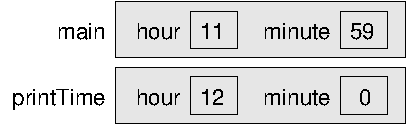
\includegraphics[scale=0.9]{figs/stack.pdf}
\caption{Stack diagram for \java{PrintTime}.}
\label{fig.stack}
\end{center}
\end{figure}

As with state diagrams, stack diagrams show variables and methods at a particular point in time.
Figure~\ref{fig.stack} is a stack diagram at the beginning of the \java{printTime} method.

%\index{scope}

%Stack diagrams help you to visualize the {\bf scope} of a variable, which is the area of a program where a variable exists.


\section{Reading documentation}
\label{sec:apidocs}

\index{documentation}

One of the nice things about Java is that it comes with an extensive library of classes and methods.
But before you use them, you might have to read the documentation.
And sometimes that's not easy.

As an example, let's look at the documentation for \java{Scanner}, which we used in Section~\ref{scanner}.
You can find it by doing a web search for ``Java Scanner''.
Figure~\ref{fig.scanner} shows a screenshot of the page.

\begin{figure}[!ht]
\begin{center}
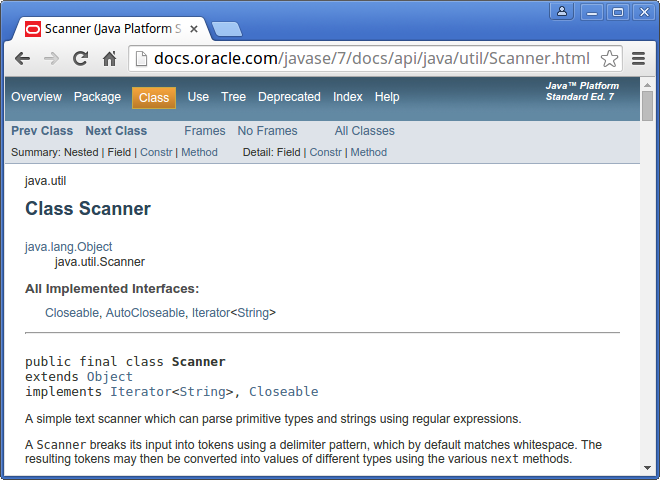
\includegraphics[width=0.9\textwidth]{figs/scanner.png}
\caption{Screenshot of the documentation for \java{Scanner}.}
\label{fig.scanner}
\end{center}
\end{figure}

Documentation for other classes uses a similar format.
The first line is the package that contains the class, such as \java{java.util}.
The second line is the name of the class.
The ``Implemented Interfaces'' section lists some of the things a \java{Scanner} can do; we won't say more about that for now.

%The next two lines indicate that every \java{Scanner} is also an \java{Object}; that will make more sense after Section~\ref{inheritance}.

The next section of the documentation is a narrative that explains the purpose of the class and includes examples of how to use it.
This text can be difficult to read because it uses terms we have not learned yet.
But the examples are often very useful.
A good way to get started with a new class is to paste the examples into a test file and see if you can compile and run them.

One of the examples shows how you can use a \java{Scanner} to read input from a \java{String} instead of \java{System.in}:

%NOTE: only use of Scanner w/o System.in; mention this again in String chapter?
\begin{code}
String input = "1 fish 2 fish red fish blue fish";
Scanner s = new Scanner(input);
\end{code}

After the narrative, code examples, and some other details, you will find the following tables:

\begin{description}

\item[Constructor summary:]
Ways of creating, or ``constructing'', a \java{Scanner}.

\item[Method summary:]
The list of methods that \java{Scanner} provides.

\item[Constructor detail:]
More information about how to create a \java{Scanner}.

\item[Method detail:]
More information about each method.

\end{description}

As an example, here is the summary information for \java{nextInt}:

\begin{stdout}
public int nextInt()
Scans the next token of the input as an int.
\end{stdout}

\index{signature}

The first line is the method's {\bf signature}, which specifies the name of the method, its parameters (none), and what type it returns (\java{int}).
The next line is a short description of what it does.

The ``Method detail'' explains more:

\begin{stdout}
public int nextInt()
Scans the next token of the input as an int.

An invocation of this method of the form nextInt() behaves in
exactly the same way as the invocation nextInt(radix), where
radix is the default radix of this scanner.

Returns:
the int scanned from the input

Throws:
InputMismatchException - if the next token does not match
    the Integer regular expression, or is out of range
NoSuchElementException - if input is exhausted
IllegalStateException - if this scanner is closed
\end{stdout}

The ``Returns'' section describes the result when the method succeeds.
In contrast, the ``Throws'' section describes possible errors and their resulting exceptions.
Exceptions are said to be ``thrown'', like a referee throwing a flag, or like a toddler throwing a fit.

It might take you some time to get comfortable reading documentation and learning which parts to ignore.
But it's worth the effort.
Knowing what's available in the library helps you avoid reinventing the wheel.
And a little bit of documentation can save you a lot of debugging.


\section{Writing documentation}
\label{sec:javadoc}

As you benefit from reading good documentation, you should ``pay it forward'' by writing good documentation.
A nice feature of the Java language is the ability to embed documentation in your source code.
That way, you can write it as you go, and as things change, it is easier to keep the documentation consistent with the code.

\index{HTML}
\index{Javadoc}

If you include documentation in your source code, you can extract it automatically, and generate well-formatted HTML, using a tool called {\bf Javadoc}.
This tool is included in standard Java development environments, and it is widely used.
In fact, the online documentation of the Java libraries is generated by Javadoc.

\index{comment!documentation}
\index{documentation!Javadoc comments}

Javadoc scans your source files looking for specially-formatted {\bf documentation comments}, also known as ``Javadoc comments''.
They begin with \java{/**} (two stars) and end with \java{*/} (one star).
Anything in between is considered part of the documentation.

Here's a class definition with two Javadoc comments, one for the class and one for the \java{main} method:

\begin{code}
/**
 * Example program that demonstrates print vs println.
 */
public class Goodbye {

    /**
     * Prints a greeting.
     */
    public static void main(String[] args) {
        System.out.print("Goodbye, ");  // note the space
        System.out.println("cruel world");
    }
}
\end{code}

The class comment explains the purpose of the class.
The method comment explains what the method does.

Notice that this example also includes an inline comment, beginning with \java{//}.
In general, inline comments are short phrases that help explain complex parts of a program.
They are intended for other programmers reading and maintaining the source code.

In contrast, Javadoc comments are longer, usually complete sentences.
They explain what each method does, but they omit details about how the method works.
And they are intended for people who will use the methods without looking at the source code.

Appropriate comments and documentation are essential for making source code readable.
And remember that the person most likely to read your code in the future, and appreciate good documentation, is you.


\section{Vocabulary}

\begin{description}

% Note: expanded definition from Chapter 1
%\term{method}
%A named sequence of statements that performs a procedure or function.
%Methods may or may not take parameters, and may or may not return a value.

\term{argument}
A value that you provide when you invoke a method.
This value must have the same type as the corresponding parameter.

\term{invoke}
To cause a method to execute.
Also known as ``calling'' a method.

\term{parameter}
A piece of information that a method requires before it can run.
Parameters are variables: they contain values and have types.

% Note: expanded definition from Chapter 2
%\term{composition}
%The ability to combine simple expressions and statements into compound %expressions and statements, making it possible to use intermediate %computations as arguments.

\term{flow of execution}
The order in which Java executes methods and statements.
It may not necessarily be from top to bottom, left to right.

\term{parameter passing}
The process of assigning an argument value to a parameter variable.

\term{local variable}
A variable declared inside a method.
Local variables cannot be accessed from outside their method.

\term{stack diagram}
A graphical representation of the variables belonging to each method.
The method calls are ``stacked'' from top to bottom, in the flow of execution.

\term{frame}
In a stack diagram, a representation of the variables and parameters for a method, along with their current values.

%\term{scope}
%The area of a program where a variable exists.

\term{signature}
The first line of a method that defines its name, return type, and parameters.

\term{Javadoc}
A tool that reads Java source code and generates documentation in HTML format.

\term{documentation}
Comments that describe the technical operation of a class or method.

\end{description}


\section{Exercises}

The code for this chapter is in the {\tt ch04} directory of {\tt ThinkJavaCode}.
See page~\pageref{code} for instructions on how to download the repository.
Before you start the exercises, we recommend that you compile and run the examples.

If you have not already read Appendix~\ref{cltesting}, now might be a good time.
It describes an efficient way to test programs that take input from the user and display specific output.


\begin{exercise}

The point of this exercise is to practice reading code and to make sure that you understand the flow of execution through a program with multiple methods.

\begin{enumerate}

\item What is the output of the following program?
Be precise about where there are spaces and where there are newlines.

{\it Hint:} Start by describing in words what \java{ping} and \java{baffle} do when they are invoked.

\item Draw a stack diagram that shows the state of the program the first time \java{ping} is invoked.

\item What happens if you invoke \java{baffle();} at the end of the \java{ping} method? (We will see why in the next chapter.)

\end{enumerate}

\begin{code}
public static void zoop() {
    baffle();
    System.out.print("You wugga ");
    baffle();
}

public static void main(String[] args) {
    System.out.print("No, I ");
    zoop();
    System.out.print("I ");
    baffle();
}

public static void baffle() {
    System.out.print("wug");
    ping();
}

public static void ping() {
    System.out.println(".");
}
\end{code}

\end{exercise}


%\begin{exercise}

%What is the difference between a variable and a method?
%In terms of their syntax, how does the Java compiler tell the difference between the two?

%%A variable is a {\em location of data}, whereas a method is a {\em location of code}.
%%In Java, methods always have parentheses, even if they have no arguments like \java{System.out.println()}.

%\end{exercise}


%ABD: We don't need this anymore since we used this as an example
%\begin{exercise}
%Draw a stack diagram that shows the state of the program in Section~\ref{time} when \java{main} invokes \java{printTime} with the arguments \java{11} and \java{59}.
%\end{exercise}


\begin{exercise}

The point of this exercise is to make sure you understand how to write and invoke methods that take parameters.

\begin{enumerate}
\item Write the first line of a method named \java{zool} that takes three parameters: an \java{int} and two \java{String}s.

\item Write a line of code that calls \java{zool}, passing as arguments the value \java{11}, the name of your first pet, and the name of the street you grew up on.
\end{enumerate}

\end{exercise}


\begin{exercise}

The purpose of this exercise is to take code from a previous exercise and encapsulate it in a method that takes parameters.
You should start with a working solution to Exercise~\ref{ex:date}.

\begin{enumerate}

\item Write a method called \java{printAmerican} that takes the day, date, month and year as parameters and that displays them in American format.

\item Test your method by invoking it from \java{main} and passing appropriate arguments.
The output should look something like this (except that the date might be different):

\begin{stdout}
Saturday, July 22, 2015
\end{stdout}

\item Once you have debugged \java{printAmerican}, write another method called \java{printEuropean} that displays the date in European format.

\end{enumerate}

\end{exercise}


\end{document}
